\chapter{Approach}
\label{sec:approach}
This section presents the approach of the proposed thesis. It starts
with the goals we want to achieve with the robot memory and a
theoretical foundation of the robot memory and how knowledge is
transferred into a knowledge based system (KBS). It follows an overview of the
architecture, which describes in which components the robot memory is
organized and how they interact with each other. Afterwards, we
describe how the implementation is planned, especially for the robot
memory and interfaces for planners, reasoners and other components.

\section{Goals}
\label{sec:goals}

This subsection presents the design goals of the robot memory:

\smallskip
\textbf{Flexible Storage and Retrieval:} The robot memory has to
provide a service for storing, updating, removing, and querying knowledge
so that different components can use the robot memory to provide knowledge,
use it as a source, or collaborate using the same memory. It should be
flexible enough to store any kind of data, information, knowledge, and
wisdom of the DIKW hierarchy in any structure. For example the robot
memory should be able to store a world model, perception results and
even large datasets, such as remembered sights of objects.

\smallskip
\textbf{Consistent Knowledge Sharing Between Knowledge Based Systems:}
The robot memory has to allow multiple components to collaborate by
consistently sharing a common database. This should especially be used
to share a common world model between different kinds of KBS. This
allows combining them with their specialized strengths
(e.g. generating plans in PDDL and executing them in CLIPS).  It
avoids inconsistencies because the basic knowledge used by the KBS is
generated by the robot memory and thus only one state estimation is
necessary. For example world model changes detected and stored in the
robot memory by CLIPS are made available to PDDL.

\smallskip
\textbf{Special Views for Different Components:} Depending on the
application of different components using the robot memory, different
views on the stored data is necessary. For example a planning
components needs another part of the stored data, than a component
learning distributions of object sights. Thus component-specific
filters are necessary. Furthermore, different components need the
stored data in different formats (e.g. depending on the used
programming language). Keys or identifiers might be named differently
and have to be translated.

\smallskip
\textbf{Knowledge Computation on Demand:} The robot memory has to
provide knowledge on demand. This is knowledge that is not stored in
the robot memory directly, but computed when needed. It allows
accessing knowledge through the robot memory that is otherwise
impracticable to compute and store continuously and for all possible
queries. For example when a component queries the distance of two
objects, it is better to compute the result on demand than to store
all distances between each two objects in the memory and to keep them
updated. Components using the robot memory should be able to provide
knowledge computation functions (\textit{computables}) to the robot
memory. This adds a lot of versatility and expandability.
%% For example it would be possible to add
%% a commonsense reasoner similar to KnowRob or ORO providing computables
%% to the robot memory. Queries for this commonsense knowledge would then
%% be forwarded to the commonsense reasoner and be solved by relating
%% knowledge in the memory to an ontology.

\smallskip
\textbf{Shared Knowledge for Multi-Robot Systems:} The robot memory
should be able to distribute parts of the knowledge over multiple
robots, which can then share a common world model necessary for
collaboration. The concept is similar to multiple planners sharing a
world model on the same machine with the difference that the
components on a multi-robot system work simultaneously and the
additional difficulty of message loss and keeping consistency. Such a
distributed robot-memory is necessary in many multi-robot domains,
especially in the RoboCup Logistics League (RCLL).
%%  where the whole robot team needs to know the world model
%% (e.g. where other robots placed intermediate products) and what other
%% robots intend to achieve at the moment.
%% If the distribution of the
%% knowledge would not be implemented in the robot memory it would have
%% to be implemented separately. 
Distributing the robot memory adds
additional requirements and challenges, especially robustness (e.g. in
the case of robots dropping out), consistency of the memory, and
accessibility so each robot can use the robot memory without large
latices.

\smallskip
\textbf{Spatio-Temporal Grounding:} It is often desirable to ground
stored knowledge based on location and time because this is the
prerequisite for many applications, such as spatio-temporal clustering
and learning distributions (e.g. at which day-times objects can be
found at which positions~\cite{deebul}). Thus the robot
memory has to be able to store knowledge tagged with spatio-temporal
information and consider this information while querying.

\smallskip
\textbf{Event Triggers:} The robot memory should be able to notify
components about relevant changes in the memory.  These notifications
are called \emph{event-triggers} and should automatically be sent
after a component registers an event it wants to be notified
about. Events include appearances of new instances of a specific
knowledge type, modifications and deletions of it, as well as
sentences becoming true or queries returning documents. The balance of
expressiveness versus performance still needs to be found. An example
use case, in which event triggers are useful, is updating reasoner
predicates.

%% \smallskip
%% \textbf{Modular Extensions:} The robot memory should be expandable
%% with modules to implement additional functionality. An example module
%% could introduce knowledge decay for removing knowledge with exceeded
%% lifetimes. This would allow differentiating short-term knowledge and
%% long-term knowledge. Other modules could, for example, reset a part of
%% the robot memory to an initial state or add confidence values to
%% stored knowledge.

\smallskip
\textbf{Persistent Storage:} To profit from long-time knowledge and to
operate robots over long time as necessary in intended domains,
such as the domestic service, the knowledge needs to be stored
persistently. This way, it is not lost when restarting a robot or
repeating an experiment depending on knowledge stored in the robot
memory.

\smallskip
\textbf{Human Interface and Visualization:} An important factor in the
development of a robotic systems is the accessibility of underlying
components for easier debugging and modeling. Therefore the robot
memory needs to provide an interface for developers to introspect and
modify the state represented in the robot memory. A visualization
would also be desirable to analyze spatio-temporal data efficiently.

\section{Theoretical Foundation}
\label{sec:formalism}
In this subsection, we lay the theoretical foundation of the robot
memory and the integration into knowledge based systems. For
this proposal, we focus on the integration into PDDL. 
The formal definition of the robot memory describes how knowledge is
represented and depends on the definition of computables. Because the
robot memory is document oriented, we first define documents and their
key-value pairs. This definition is derived from the specification of
the Binary JavaScript Object Notation
(BSON)\footnote{\url{http://bsonspec.org/spec.html}} used in MongoDB.
Because documents can be nested, we define them by induction. Unnested
documents are defined as follows:
\begin{enumerate}
\item \textbf{Keys} are strings $\mathcal{K} := \Sigma^*$, where
  $\Sigma$ contains all valid characters.
\item  \textbf{Atomic values} $\mathcal{V}_0$ is a countable infinite set of constants with
  integers, floating point numbers, and strings.
\item \textbf{Unnested key-value pairs:} $\mathcal{P}_0:=\mathcal{K}\times\mathcal{V}_0$
\item \textbf{Unnested documents} are sets of key-value pairs with
  unique keys and thus included in the power set of $\mathcal{P}_0$:\\
  $\mathcal{D}_0:=\{
  d\in\mathbb{P}(\mathcal{P}_0)|
  \forall (k,v),(k',v')\in d , k\neq k' \vee (k,v)=(k',v')
  \}$
\end{enumerate}
Values and documents with a nesting depth up to $n$ with $n>=1$ can be
defined as follows:
\begin{enumerate}
\item  \textbf{Values:} $\mathcal{V}_n := \mathcal{V}_{n-1} \cup \mathcal{D}_{n-1}$
\item \textbf{Key-value pairs:} $\mathcal{P}_n:=\mathcal{K}\times\mathcal{V}_n$
\item \textbf{Documents:}
  $\mathcal{D}_n:=\{
  d\in\mathbb{P}(\mathcal{P}_n)|
  \forall (k,v),(k',v')\in d , k\neq k' \vee (k,v)=(k',v')
  \}$
\end{enumerate}
This yields the set of all \textbf{finitely nested documents}
$\mathcal{D}=\cup_{n\in\mathbb{N}}\mathcal{D}_n$.
The set of all values is $\mathcal{V}=\cup_{n\in\mathbb{N}}\mathcal{V}_n$.
  Infinite nesting and
documents containing themselves are not considered because they can
not properly be mapped into most KBS formalisms.
\\
A \textbf{database} is a finite set of documents $\mathcal{DB} \subset \mathcal{D}$.
%% with unique object
%% identifiers, which are a special key-value pair:
%% \begin{align*}
%% \mathcal{DB} \subset & \{d\in\mathcal{D} | ("\_id",v)\in d\},\\
%% & \text{where } \forall d,d' \in \mathcal{DB} \text{ with } ("\_id",v)\in
%% d \text{ and } ("\_id",v')\in d' , d=d' \vee v\neq v'
%% \end{align*}
\textbf{Queries} are represented by documents $q\in\mathcal{D}$ and yield a set
of documents $r\subseteq\mathcal{DB}$ as result when executed in a database according a
specification (e.g. of MongoDB~\cite{mongodb}). For example, the query
$\{("object","cup"),("room","kitchen")\}$ yields all documents containing these
key-value pairs and thus all cups in the kitchen.
\\
A \textbf{computable} $f$ is a function mapping a query document to a
set of computed documents
$$f: \mathcal{D} \rightarrow \mathbb{P}(\mathcal{D})\text{.}$$
The component providing the computable has to ensure that the function is computable and terminates.
%
With these preliminaries, we can now define a \textbf{robot memory} as tuple
of a database~$\mathcal{DB}$ and a set of computables~$\mathcal{C}$:
$$\mathcal{RM}=(\mathcal{DB},\mathcal{C})$$
%
The set of documents \textbf{memorized} by the robot memory consists
of the underlying database and all computable documents:
$$mem(\mathcal{RM})=DB \cup \bigcup_{f\in\mathcal{C}}f(\mathcal{D})$$

To integrate the robot memory into PDDL, we need to define the
\textbf{mapping functions} $map_d$ between documents and predicates, and
$map_v$ between values and terms. As prerequisite, the connection
between key-names in documents and predicates, functions, and their
attributes needs to be defined. Let $\mathcal{R}$ be the \textbf{set
  of predicate symbols} and $\mathcal{F}$ be the \textbf{set of function
  symbols}, then
%
$$name_{pred}: \mathcal{R} \rightarrow \Sigma^*
\text{ and } name_{func}: \mathcal{F} \rightarrow \Sigma^*$$
%
map to the strings used in document keys
(e.g. $name_{pred}(\text{at})="\text{at}"$). To ensure unambiguity,
$name_{pred}$ and $name_{func}$ should
be injective and their images disjunctive. The functions
%
$$ name_{func-atr}: \mathcal{R} \times \mathbb{N} \rightarrow
\mathcal{K} \text{ and } name_{pred-atr}: \mathcal{F} \times \mathbb{N}
\rightarrow \mathcal{K}$$
%
map the attributes in the predicate or function to a key
name (e.g. $name_{pred-atr}(\text{at},1)="\text{object}"$ and
$name_{pred-atr}(\text{at},2)="\text{room}"$).
\\
Now we can define the mapping of values in documents to terms as
follows. Values that are no sub-documents can be mapped directly to
the corresponding constant:
$$map_f(v)=v, v \in \mathcal{V}_0$$
Otherwise the value is a sub-document, which is mapped to a function term:
\begin{align*}
  map_f(d)= &\text{ }f(map_f(v_1), ..., map_f(v_n)), \text{ iff } f \text{ is a n-array function in } \mathcal{F},\\
  &("function", name_{func}(f))\in d,
  \forall i \in \{1..n\} (name_{func-atr}(f,i), v_i)\in d\\
  map_f(d)= &\text{ } nil_f, otherwise\text{~~~~~~~~~~~~~~~}
\end{align*}
where $nil_f$ is a new constant used for not mappable documents.
Similarly documents can be mapped to predicates as follows:
\begin{align*}
  map_p(d)=&\text{ }p(map_f(v_1), ..., map_f(v_n)), \text{ iff } p \text{ is a n-array predicate in } \mathcal{R},\\
  &("predicate", name_{pred}(p))\in d,
  \forall i \in \{1..n\} (name_{pred-atr}(p,i), v_i)\in d\\
  map_p(d)=& \text{ }nil_p, otherwise\text{~~~~~~~~~~~~~~~}
\end{align*}
For example is
\begin{align*}
map_p&(\{("predicate", "at"),("object", "cup"),("room",
"kitchen")\})\\
&= at(map_f("cup"), map_f("kitchen")) = at(cup, kitchen) \text{.}
\end{align*}
\todo{other direction: parse resulting plan}
This theoretical foundation of the robot memory and the mapping of
queried documents into predicates is the basis for the generation of
PDDL problem descriptions. In future work, this can also be used to
formalize the integration of the robot memory into Golog, but this
exceeds the scope of the proposed thesis.

\section{Architecture}
\label{sec:arch}
This subsection presents the architecture of the robot memory and
explains its design considerations. It shows how the intended
functionality is organized in smaller components and how these
components interact with each other. The architecture contains
standard concepts of software engineering, most importantly a layered
architecture, functional abstraction, and data
abstraction~\cite{software-architecture} to allow
reusability and adaptability to changing requirements and use cases.
%% functional abstraction,
%% %% (e.g. of the different processes happening during storing and
%% %% querying)
%% and data abstraction.
%% %%  (e.g. of stored knowledge which is
%% %% more specialized internally than visible from a using
%% %% application)

\reffig{fig:arch} shows the architecture of the robot
memory and is explained in the following.
\begin{figure}
  \centering
  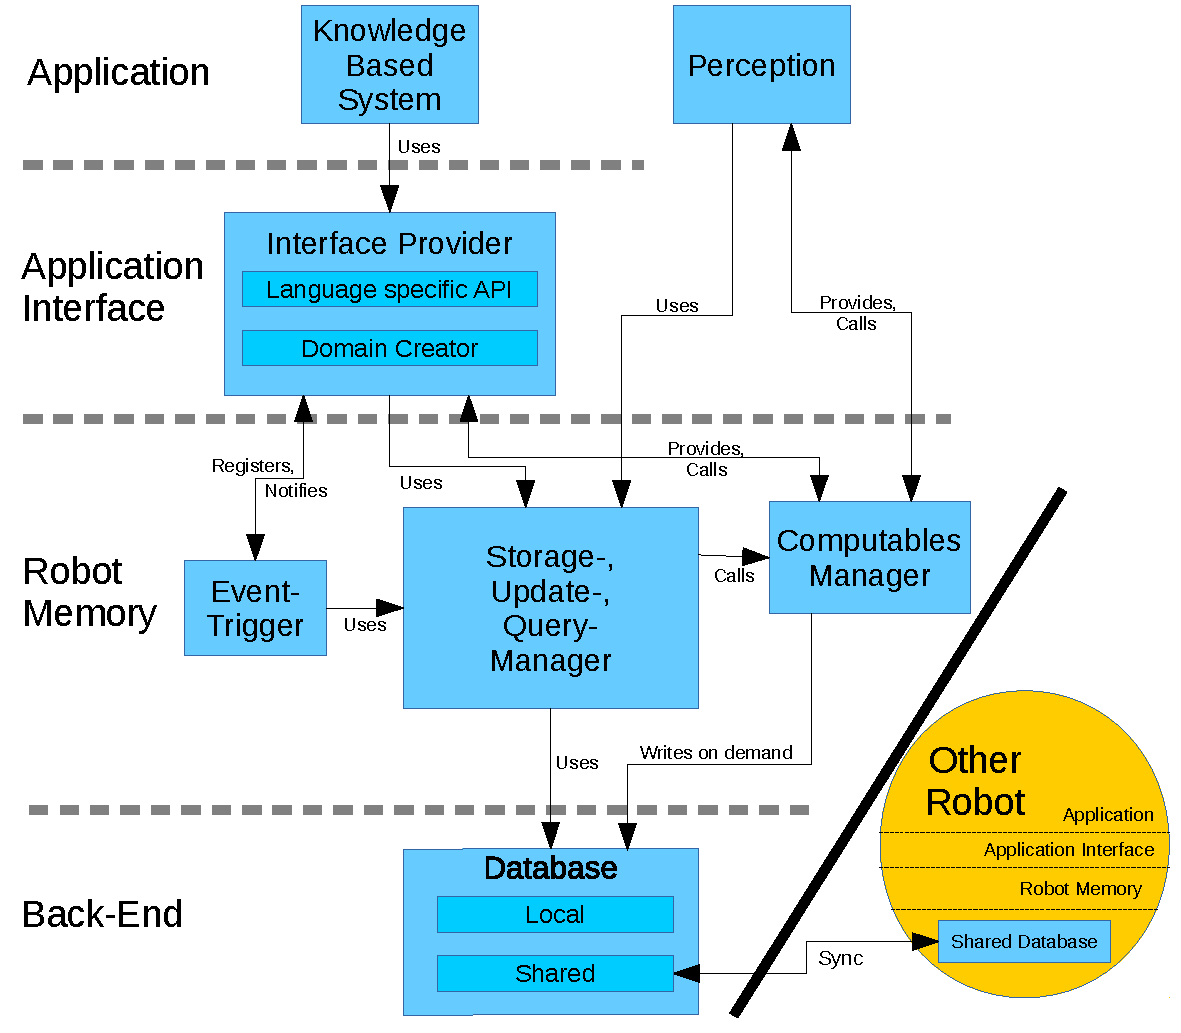
\includegraphics[width=0.9\textwidth]{architecture.pdf}
  \vspace{-5mm}
  \caption{Software architecture of the Robot Memory}
  \label{fig:arch}
  \vspace{-5mm}
\end{figure}
The architecture organizes all components into four layers: Back-End,
Robot Memory, Application Interface, and Application. The Back-End
contains a database for storing knowledge and executing
queries. There is a private part and a shared part distributed between
multiple robots using the same architecture. This distribution can
utilize the replication features of the database. The Robot
Memory-layer contains the central functions that distinguish the robot
memory from a pure database. It contains the Storage-, Update-, and
Query-manager, which is an intermediate component that realizes most of
the robot memory's functionality by modifying and enhancing queries,
storage, and update requests before applying them to the database. If a
query asks for knowledge provided by a computable, the manager forwards it to the
computable manager, which manages which computable is provided by
which application and requests the computation on demanded. The
component responsible for event-triggers receives and manages
registrations of applications that want to be notified in the case of
an event. It uses the Query-manager to check if events happen and
notifies applications accordingly. Additionally the Storage-, Update-,
and Query-manager can initialize the robot memory (e.g. to setup the
world model for a new RCLL game).
%% These extensions can use the Command Pattern~\cite{design-patterns}
%% and to work process compositionally and dynamically.
Between the robot memory and a planner or reasoner components is the
Application Interface layer. For each KBS, it includes a
Interface Provider component, which makes the function of the robot
memory available to the KBS and the special programming language
used. It is not necessary for components that can directly use the C++
interface of the robot memory. The responsibilities of the interface
provider also include transforming query results in the appropriate
format used by the KBS and eventually renaming key-names if they
have be mapped to match the names used in the KBS
model. Because languages and concepts of knowledge based systems can be
very different, each KBS needs a separate Interface
Provider. The Interface Provider can also contain a domain creator,
which creates an initial state (e.g. a problem definition or initial
fact base) from a template and additional knowledge resulting from
queries. Finally the Application layer contains all components using
the robot memory either through the Interface provider or directly
through the robot memory interface. Application components can also
register event-triggers and provide computation functions for
computables. The sources and consumers of knowledge stored in the
robot memory are the applications using it. The ordinary data flow
starts in the application requesting storage, modification, or
querying of knowledge (over the language specific interface). The
Storage-, Update-, and Query-manager forwards the request enhanced
with management information to the database. For queries, the result
is transferred back on the reversed path of the query request. For
computables, the only difference in the data flow is the knowledge
computation before executing the query in the database. The Storage-,
Update-, and Query-manager additionally initiates the knowledge
computation via the Computables Manager, which forwards the query to
the application providing the specific computable. The application
then computes and stores the result in the robot memory, where it is
queried afterwards.
%% Additionally the Initializer module can
%% provide the initial knowledge from a file (e.g. for the world model of
%% a new RCLL game).


\section{Implementation}
\label{sec:impl}
This subsection covers the considerations for the implementation. It is
separated according to the layered architecture. Both application
layers are represented by the planner and reasoner part, because all
other application components (e.g. for perception) can simply use the
C++ interface of the robot memory.

\subsection{Back-End}
\label{sec:back-end}
The back-end is realized with MongoDB. It acts as storage of the robot
memory, and executes queries. The representation of stored knowledge
utilizes the document structure of MongoDB with key-value pairs and
nested sub-documents. This allows a very flexible storage of
knowledge-pieces in the structure induced by the application and
expandable by robot memory information.

\begin{wrapfigure}{r}{0.47\textwidth}
  \vspace{-0.8cm}
\begin{lstlisting}[style=SmallJSON,
  caption={Representation of a knowledge piece in the back-end},
  label=lst:backend,
  framexleftmargin=1pt, xleftmargin=0pt,
 morekeywords={}, numbers=none]
 {
   _robot_memory_info:
   {
     persistent: true,
     decay_time: ISODate(
       "2016-05-19T 23:50:00.000Z")
   },
   type: "object info",
   name: "milk_1",
   position: {x:2.5, y:1.0, z:0.0},
   storage_place: "refrigerator"
 }
\end{lstlisting}
\vspace{-14mm}
\end{wrapfigure}
An example document stored in the back-end is shown in
\reflst{lst:backend}.  It contains knowledge about a bottle of milk as
it could be needed by a planner with additional information where it
should be stored later. Additionally the document contains meta
information needed by the robot memory (e.g. if the document should be
stored persistently or removed at restart and when it should be
dropped because it's use-time has expired). The MongoDB back-end also
manages the distribution of knowledge between multiple robots. A part
of the robot memory is only locally relevant. The other part that
should be shared has to be set up as MongoDB replica set as already
described in \refsec{sec:mongodb}. This ensures that efficient
networking code is used. The other problems of a distributed database,
such as consistency, master election, and synchronization are solved
by MongoDB using replication. The back-end also contains the
operations log (oplog) of MongoDB, a separate
%% capped
collection containing a list of changes to the database with a
timestamp. This can be accessed by the robot memory to analyze
changes for event-triggers.

\subsection{Robot Memory}
\label{sec:impl-memory}
The robot memory middle-layer implements most functions exceeding a
typical database.
%% between the
%% applications storing and querying knowledge and the MongoDB back-end
%% is an important part of the thesis because most of the functions
%% exceeding a typical database are realized here.
A central question is which query language should be used between
applications and the robot memory because this determines the
expressiveness and has a large impact on the performance. We choose to
use the query language of MongoDB as it is already used between the
robot memory and the back-end. This has many advantages compared to
using other query languages, such as SQL, SPARQL,
XQuery~\cite{query-languages}, and JSONiq~\cite{jsoniq}.
\todo{move into conceptual part}
%
For the application view, the query language of MongoDB is a good
choice because it is an intuitive query language, has been proven as
efficient for usual and well designed queries, and is also highly
expressive when using additional JavaScript functions or the MapReduce
paradigm~\cite{mongodb,RoboDB}. For the robot memory, it requires no
translation before application on the database and is very flexible
for extending and modifying queries because queries are structured as
documents with key-value fields and can be nested or executed in
sequence. Furthermore, MongoDB queries can easily be parsed (e.g. from
a string) by using the MongoDB C++ API. The resulting object can be
analyzed and modified for example to add key-value pairs or to check
if computables are queried.

This provides the starting point for the Storage-, Update-, and
Query-manager. When adding new documents, the
\texttt{robot\_memory\_info} sub-document can be added to store
additional meta information. When querying documents, this information
can be removed by using a filter. To detect queries for computables,
the manager can analyze the fields of the query to check if there is a
computable provided for it.  For example when a query contains the
field \texttt{type:"distance"} and there is a application that
provides computation functions for distances between two objects, the
query can be forwarded with the additional parameters, the two
objects.  When some fields are missing (e.g. only one object is given)
the application may have to compute all distances, so that the query
can afterwards be executed on the set of results (e.g. to find the
nearest one with some property). To execute the query as a usual query
with arbitrary filters, aggregation, and functions, the computation
function writes the result into a separate collection the query
can be executed on with MongoDB. To lower the computational effort of
processing the same query frequently it would be possible to add
time-bounded caching for computed knowledge. We have verified this
concept of computables using a prototype, which executes queries from
interface messages either on the MongoDB directly or in case of
computables about other interfaces, generates the knowledge from the
blackboard on demand and then executes the query.

To implement event-triggers, a registration function needs to be
provided that takes a notification function and a query to define the
event. This query can check the oplog first whether there are changed
documents with relevant key-value pairs and afterwards execute a more
complex query on the database. The registration also specifies whether
the callback function is called if the query result changes, returns
no document, or is not empty. Whether event-triggers on computables
perform well, has to be evaluated. It would be possible to allow
events only on knowledge in the database or to compute the knowledge
and check for the event in certain intervals while monitoring the
computation time.

%% The robot memory . For
%% implementation, they can be called periodically or with hook-points at
%% major steps of the robot memory such as initialization and query
%% execution. For example, a knowledge decay module could use cronjob to
%% remove documents with exceeded lifetimes in certain intervals. Further
%% hook-points would be at query-modification time (e.g. to add
%% additional meta-information) and at query-result-return time (e.g. to
%% filter or modify resulting documents).

\subsection{Planner/Reasoner}
\label{sec:impl-planner}
The implementation on the application layer includes the development
of the Interface Provider and the usage of the robot memory in the
planning language. As an example for the various planners and
reasoners, we focus here on CLIPS. The Interface Provider for CLIPS
can be realized as CLIPS-feature in Fawkes as it was already done for
providing CLIPS access to the blackboard, Protobuf-messaging and the
navgraph. The CLIPS \emph{robot-memory feature} will be implemented in C++
and provides the CLIPS environment with functions that call C++
functions of the robot-memory feature. For example \reflst{lst:clips-rm}
\begin{figure}
  \begin{lstlisting}[showlines,style=ReallySmallCLIPS, caption={CLIPS function to execute a query},
  label=lst:clips-rm,
  emph={skill, args, state, target, res},
  emphstyle=\bfseries\color{green!80!black},
  emph={[2]\?skill, \$\?args, wait-for-lock, \?target, use,
  WAIT-FOR-LOCK, SKILL-EXECUTION, running},
  emphstyle={[2]\bfseries\color{blue!80!black}},
  morekeywords={retract, assert, modify, skill-call, skill-to-execute,
    wait-for-lock}]
(rm-query "database.collection"
          (str-cat "{type:'order', end-time:{$gt:" ?gametime "}}"))
\end{lstlisting} %$ This is just to fix Emacs highlighting due to dollar sign in code above
\end{figure}
would be the CLIPS function, which queries all orders that have not
ended yet, by creating the query using string concatenation to fill in
the current game-time. The result would be a list of pointers to document
objects represented as instances of CLIPS templates. Similarly there
can be functions for registering events and providing computables.

The Domain Creator for CLIPS can be implemented by creating the initial
fact-base with a static list of facts and additional facts resulting
from a set of queries. For example, a domain creator implemented in
the CLIPS language could execute the query function in
\reflst{lst:clips-rm} and assert all orders as facts into the fact
base.
%% possibility to also generate rules form robot memory

CLIPS could use event-triggers to be notified when there is a new PDDL
plan in the robot memory that should be executed or when the world
model has changed in the robot memory and thus facts in CLIPS have to
be updated.

\chapter{Evaluation}
\label{sec:eval}
This section covers the evaluation of the proposed thesis. We will
evaluate the robot memory qualitatively in both application domains,
the RCLL and RoboCup@Home league, and quantitatively.

The qualitative evaluation analyzes how well the robot memory can be
used, how useful it is, and where difficulties are. It also includes
analyzing the expressiveness and convenience of representing and
querying knowledge, the integration into KBS
languages, and the shared access to the robot memory across different
applications and robots. To perform the qualitative evaluation, we
will implement prototypes using main features of the robot
memory. These prototypes act as proof of concept without implementing
complete domain solutions which would extend the scope of the thesis.
%
The general storage and query features of the robot memory will be
evaluated in the RCLL context with a CLIPS agent that stores the world
model in the robot memory and keeps it up to date. This shows how well
the robot memory can be integrated in a reasoner.
%
In a second step, the world model should be synchronized between a
multi-robot team to evaluate how well the shared robot memory works in
a distributed system. This includes an analysis of the network
throughput and robustness to package loss.
%
The planner specific view of the robot memory will be evaluated with a
PDDL planner in the RCLL domain. The robot-memory-PDDL interface
should generate a PDDL problem description from a world model stored
in the robot memory. The resulting plan should be stored in the robot
memory and queryable by CLIPS.
%
To evaluate event-triggers, we will register events depending on
changes of the RCLL world model that need to be updated in the local
CLIPS agent. Furthermore we want to try more complex events, which
could be used to trigger actions in the @Home domain (e.g. the space
occupied by objects in the dishwasher is high enough to start it).
This should show how useful and expressive registered events can be.
% 
These prototypes should show if the robot memory allows knowledge
sharing between multiple KBS. A related thesis,
which is in preparation, wants to utilize PDDL for global task
planning and CLIPS for execution to achieve more efficient multi-robot
behavior in the RCLL. It could benefit from using the robot memory and
yield further evaluation results.

To further evaluate how well the robot memory works in a hybrid
reasoning context with motion planners and symbolic planners, we will
also develop a RoboCup@Home related prototype using computables. Here
the robot memory should hold knowledge usable by a motion planner and
transform it into symbolic knowledge usable by a reasoner (e.g. if the
robot's coordinates are stored and a reasoner asks for the room the
robot is in). Thus a computable has to compute the symbolic knowledge
from the spatio-temporal one or vice versa. Quantitatively,
computables have to be evaluated by comparing the times between giving
the query and receiving the results with and without computables
taking the computation time, either on demand or on changing data.

To analyze how the query computation time increases with increasing query
expressiveness and database scale, we want to implement a simple
tidying up scenario. The robot memory models a scene with current
object placements and object storage positions in increasing
amount. The queries start simple (e.g. where is the storage place for
the red cup) and get more complex (e.g. which objects are not at their
storage position). Furthermore, the CPU and memory usage of the robot
memory have to be analyzed as well as the size of the database on the
hard drive.

\chapter{Conclusion}
\label{sec:conclusion}
In the proposed master thesis, we develop the conceptual and
architectural design of a generic robot memory and implement it in
Fawkes with MongoDB. The envisioned robot memory is a generic,
capable, and efficient long-time storage for knowledge, which is the
basis for memorizing a complex environment and thus for reasoning in
it. The robot memory is a knowledge sharing system, on the one hand,
for multiple knowledge based systems and, on the other hand, for
multiple robots working collaboratively. Therefore it allows a
consistent and tight integration of planners and reasoners while
avoiding multiple state estimations. The robot memory is a hybrid
reasoning tool that allows storing spatio-temporal knowledge and
transforming it on demand into symbolic knowledge.

In contrast to existing knowledge processing systems, such as KnowRob
and ORO, the concept of the robot memory decouples the storage of
knowledge and reasoning on it and is based on a document-oriented
representation. As we want to show in the evaluation of the thesis,
this allows more efficient and scalable querying and tighter
integration of multiple KBS and robots teams.

The architecture of the robot memory builds on top of a database
system. It contains components for dispatching and enhancing queries
and storage requests, for knowledge computed on demand, and for
event-triggers notifying about changes. There are interface
components, which provide the functionality of the robot memory for
KBS by giving access in the used languages and transforming query
results into the appropriate form. Applications using the robot memory
can store and query knowledge, provide computables for other
components, and use event triggers.

Challenges of the thesis include the conceptual tuning of the
document-oriented knowledge representation and querying to achieve a
balance between expressiveness and computation time. Further
challenges are the design of computables in a document-oriented system
to allow on demand computation of knowledge in an efficient and still
powerful way, and the robust knowledge sharing in a distributed
multi-robot system.

The main part of the thesis focuses on the robot memory as back-end of
a robot system and foundation for future applications, such as a
thesis in preparation about global PDDL planning in the RCLL with
CLIPS as executive. Nevertheless we will use the RCLL and RoboCup@Home
application domains to implement prototypes utilizing the robot memory
and working as proof of concept for qualitative evaluation and basis
for quantitative evaluation. For these two application domains, we
will connect the robot memory to CLIPS, PDDL, and various perception
components.

\section{Schedule}
\begin{table}
  \centering
  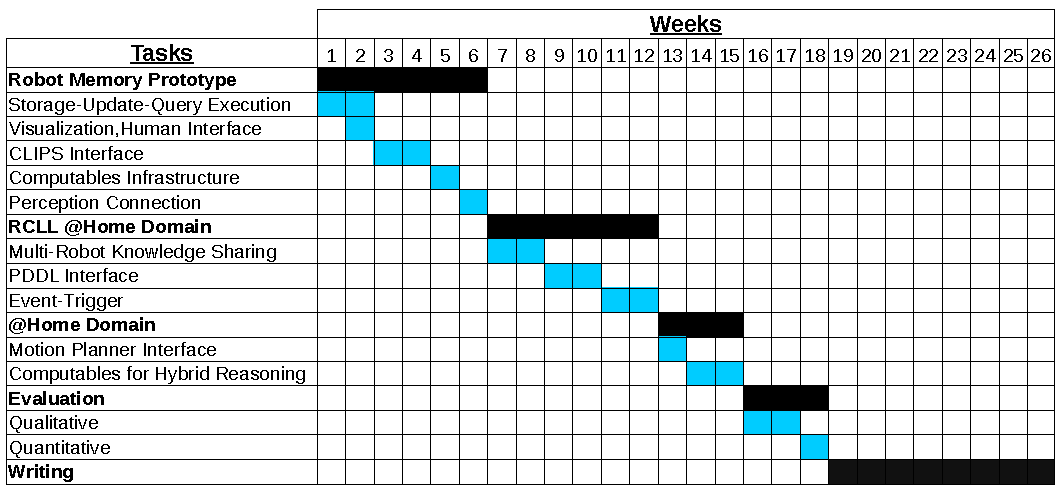
\includegraphics[width=\textwidth]{gantt-chart}%
  \vspace{-5mm}
  \caption{Gantt Chart of the thesis time schedule}
  \label{tab:gantt}
\end{table}
The time-schedule of the thesis is shown in \reftab{tab:gantt}. The
first part focuses on developing a robot-memory prototype with the
CLIPS interface, infrastructure for computables, and fundamental
connection to perception components. This prototype is then
iteratively improved to implement all other features needed in the
RCLL and in RoboCup@Home domain. The robot-memory itself and both
applications are then evaluated and the rest of the time is spent on
the written report.
